\section{Experiments}
In order to experiment the proposed method, we first collected a dataset guided by the human preferences captured via the statistics of a popular online recipe collection --WikiHow \cite{wikiHow}--. After collecting the dataset, we labelled small part of the dataset with frame-wise activity labels and used the resulting set as an evaluation corpus. Neither the set of labels, nor the temporal boundaries are exposed to the competing algorithm since the set-up is completely unsupervised. We experiment our algorithm against the set of unsupervised clustering baselines and state-of-the-art algorithms from video summarization literature which are applicable. In the rest of this section, we first explain the dataset we collected and labelled in detail. Then, we explain the method which we compare our method against. After explaining the metrics we use, we give both qualitative and quantative results. Due to the space limitation, we defer some of the results to the supplementary metarial.

\subsection{Dataset}
We guide our datacollection effort with human preferences based on WikiHow \cite{wikiHow} statistics. After obtaining the top100 queries people interested in WikiHow, we chose top25 ones which are directly related to the physical world and objects. We ignore the queries like \emph{How to get over a break up‏?‎} and \emph{How to write a resignation Letter?}. Resulting 25 queries are;


\emph{\textbf{How to}}\footnotesize
\emph{Bake Boneless Skinless Chicken, Cook Steak in a Frying Pan, Make Jello Shots, Tell if Gold Is Real, Bake Chicken Breast, Hard Boil an Egg, Make Pancakes, Tie a Bow Tie
Broil Steak, Make a Grilled Cheese Sandwich, Make Scrambled Eggs, Tie a Tie, Clean a Coffee Maker, Make a Milkshake, Make Yogurt, Unclog a Bathtub Drain, Cook an Omelette,
Make a Smoothie, Poach an Egg, Cook Lobster Tails, Make Beef Jerky, Remove Gum from Clothes, Cook Ribs in the Oven, Make Ice Cream, Tell if an Egg is Bad}
\normalsize

For each of the recipe, we queried YouTube and crawled the top 100 videos. We also downloaded the english subtitles if they exist. For evaluation set, we choose 5 videos out of 100 per query. Hence, we have total of 125 evaluation videos and 2375 unlaballed videos. We also realease the collect dataset at \url{http://anonymous.edu/MMRecipe}.

\subsection{Qualitative Results}
\begin{figure}
  \begin{subfigure}[b]{0.5\textwidth}
  \includegraphics[width=\textwidth]{act_gt}
  \caption{Ground Truth Activity Labels}
  \end{subfigure}
  \begin{subfigure}[b]{0.5\textwidth}
  \includegraphics[width=\textwidth]{act_our}
  \caption{Activity Labels extracted by Our Method}
  \end{subfigure}

\begin{subfigure}[b]{0.5\textwidth}
\begin{subfigure}[b]{0.5\textwidth}
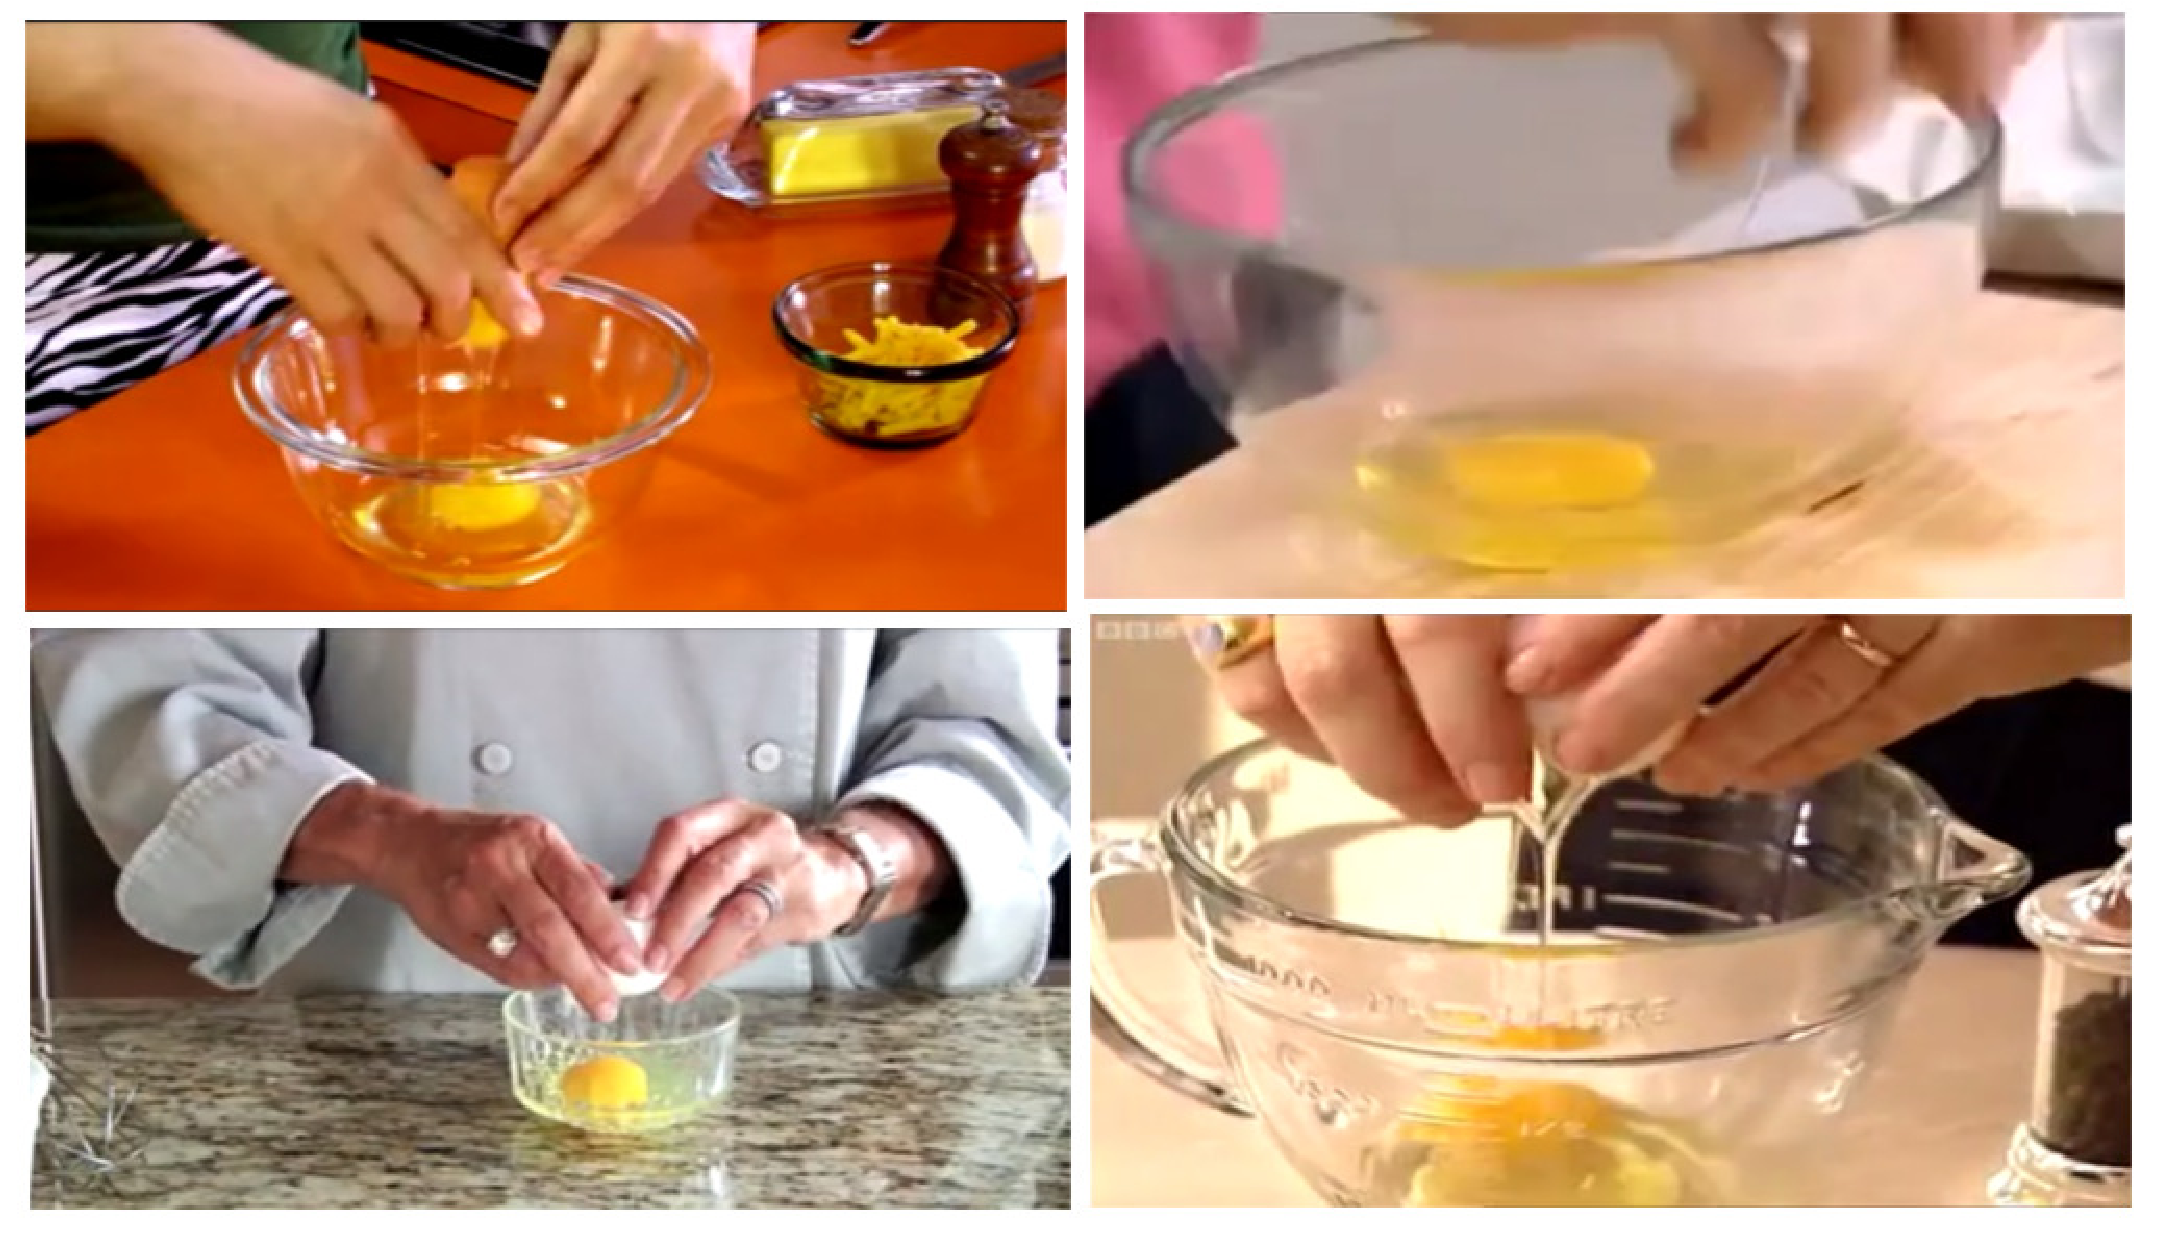
\includegraphics[width=\textwidth]{cred}
\color[HTML]{FF3800}{Crack the eggs one at a time into a bowl.}
\end{subfigure}~
\begin{subfigure}[b]{0.5\textwidth}
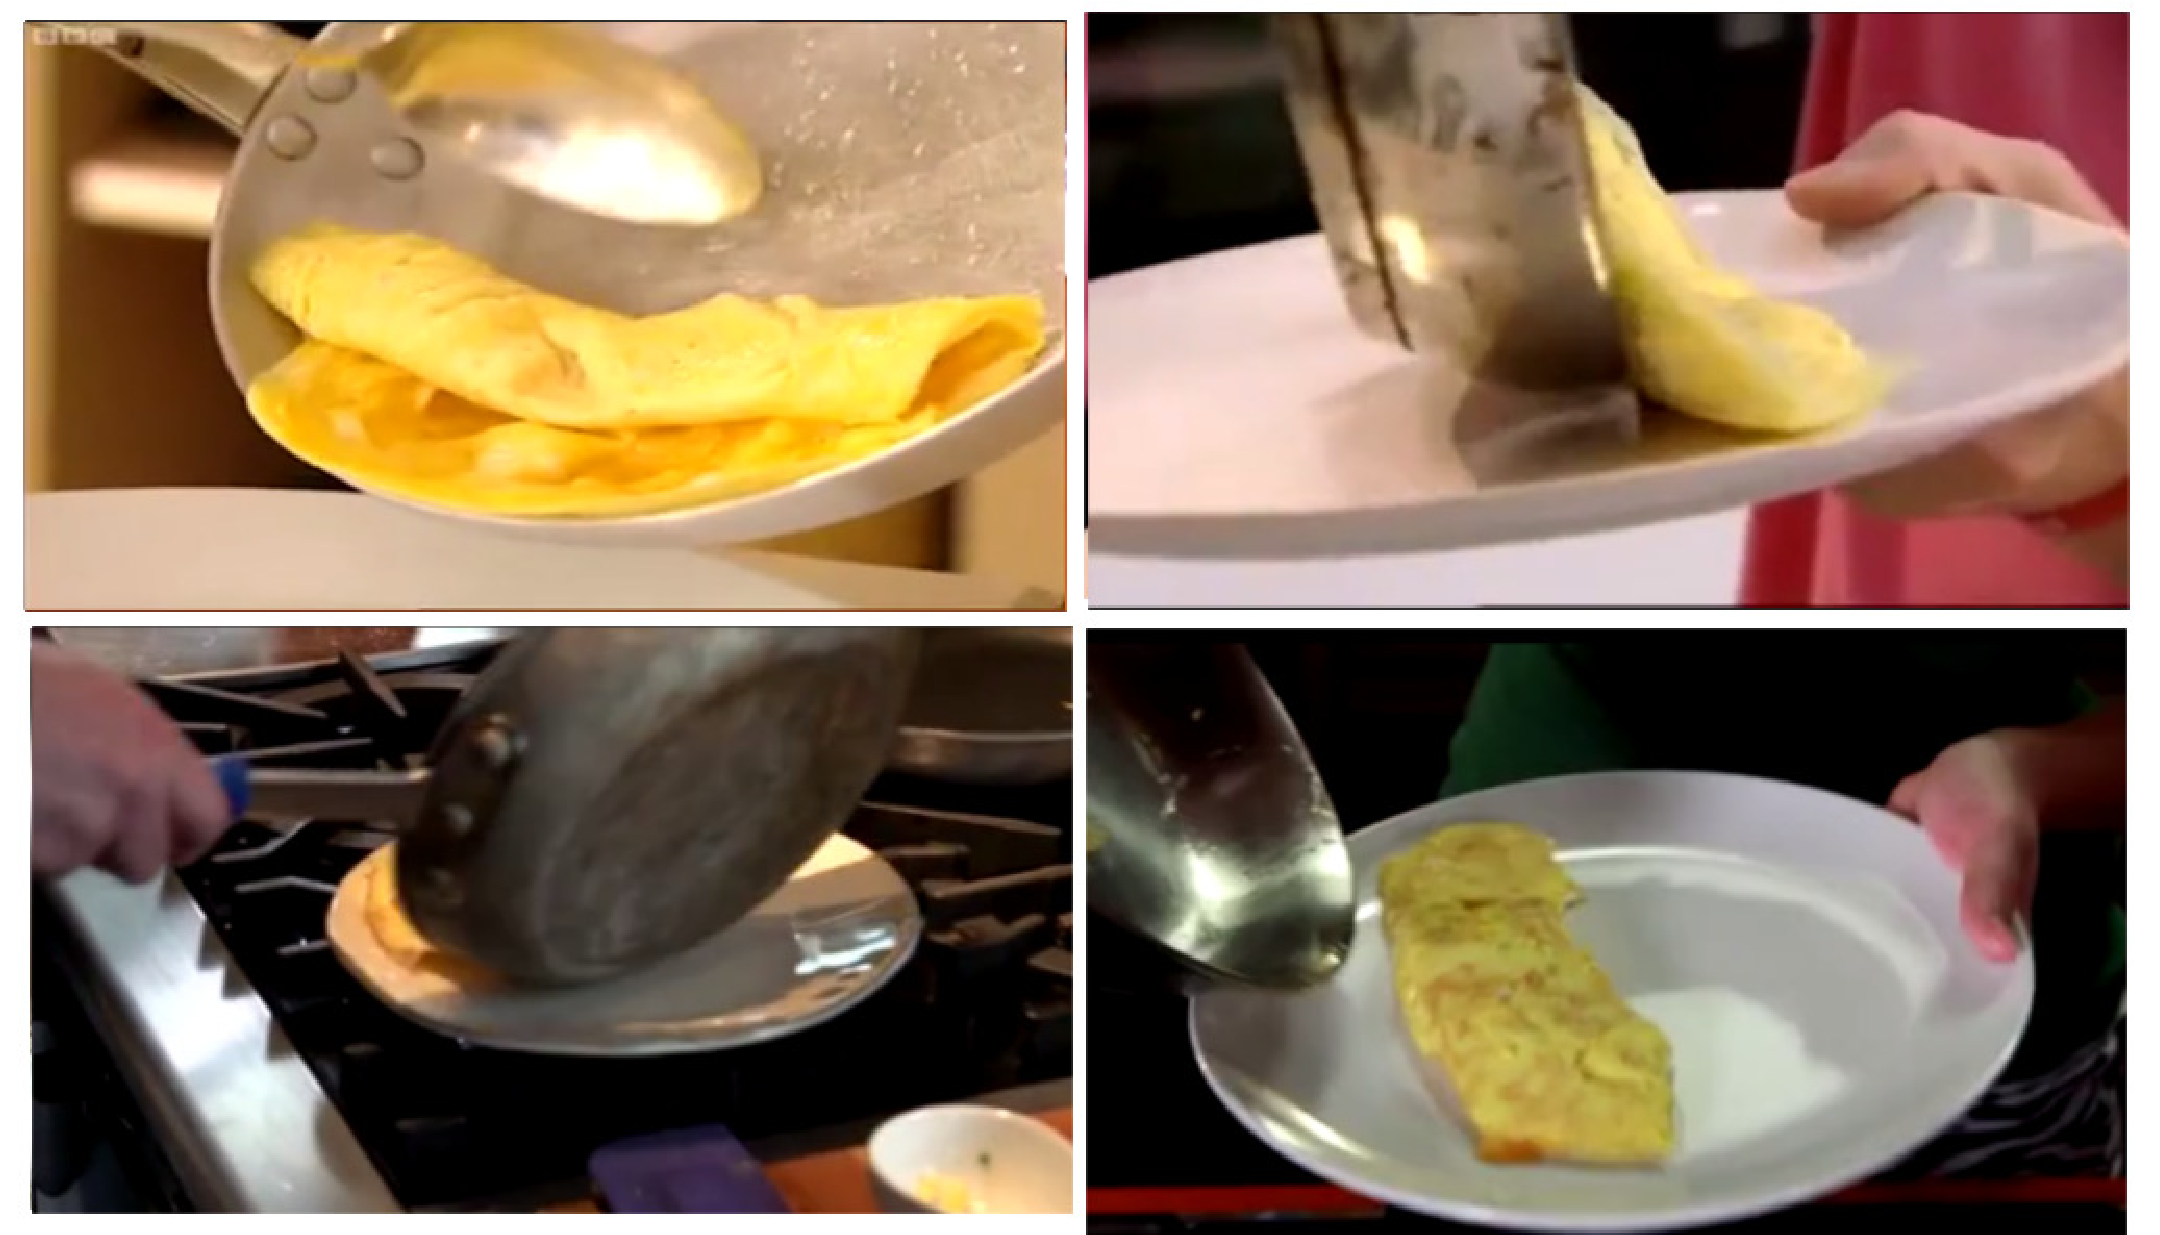
\includegraphics[width=\textwidth]{cyan}
\color[HTML]{00FFED}{Remove the omelette onto a plate.}
\end{subfigure}


\begin{subfigure}[b]{0.5\textwidth}
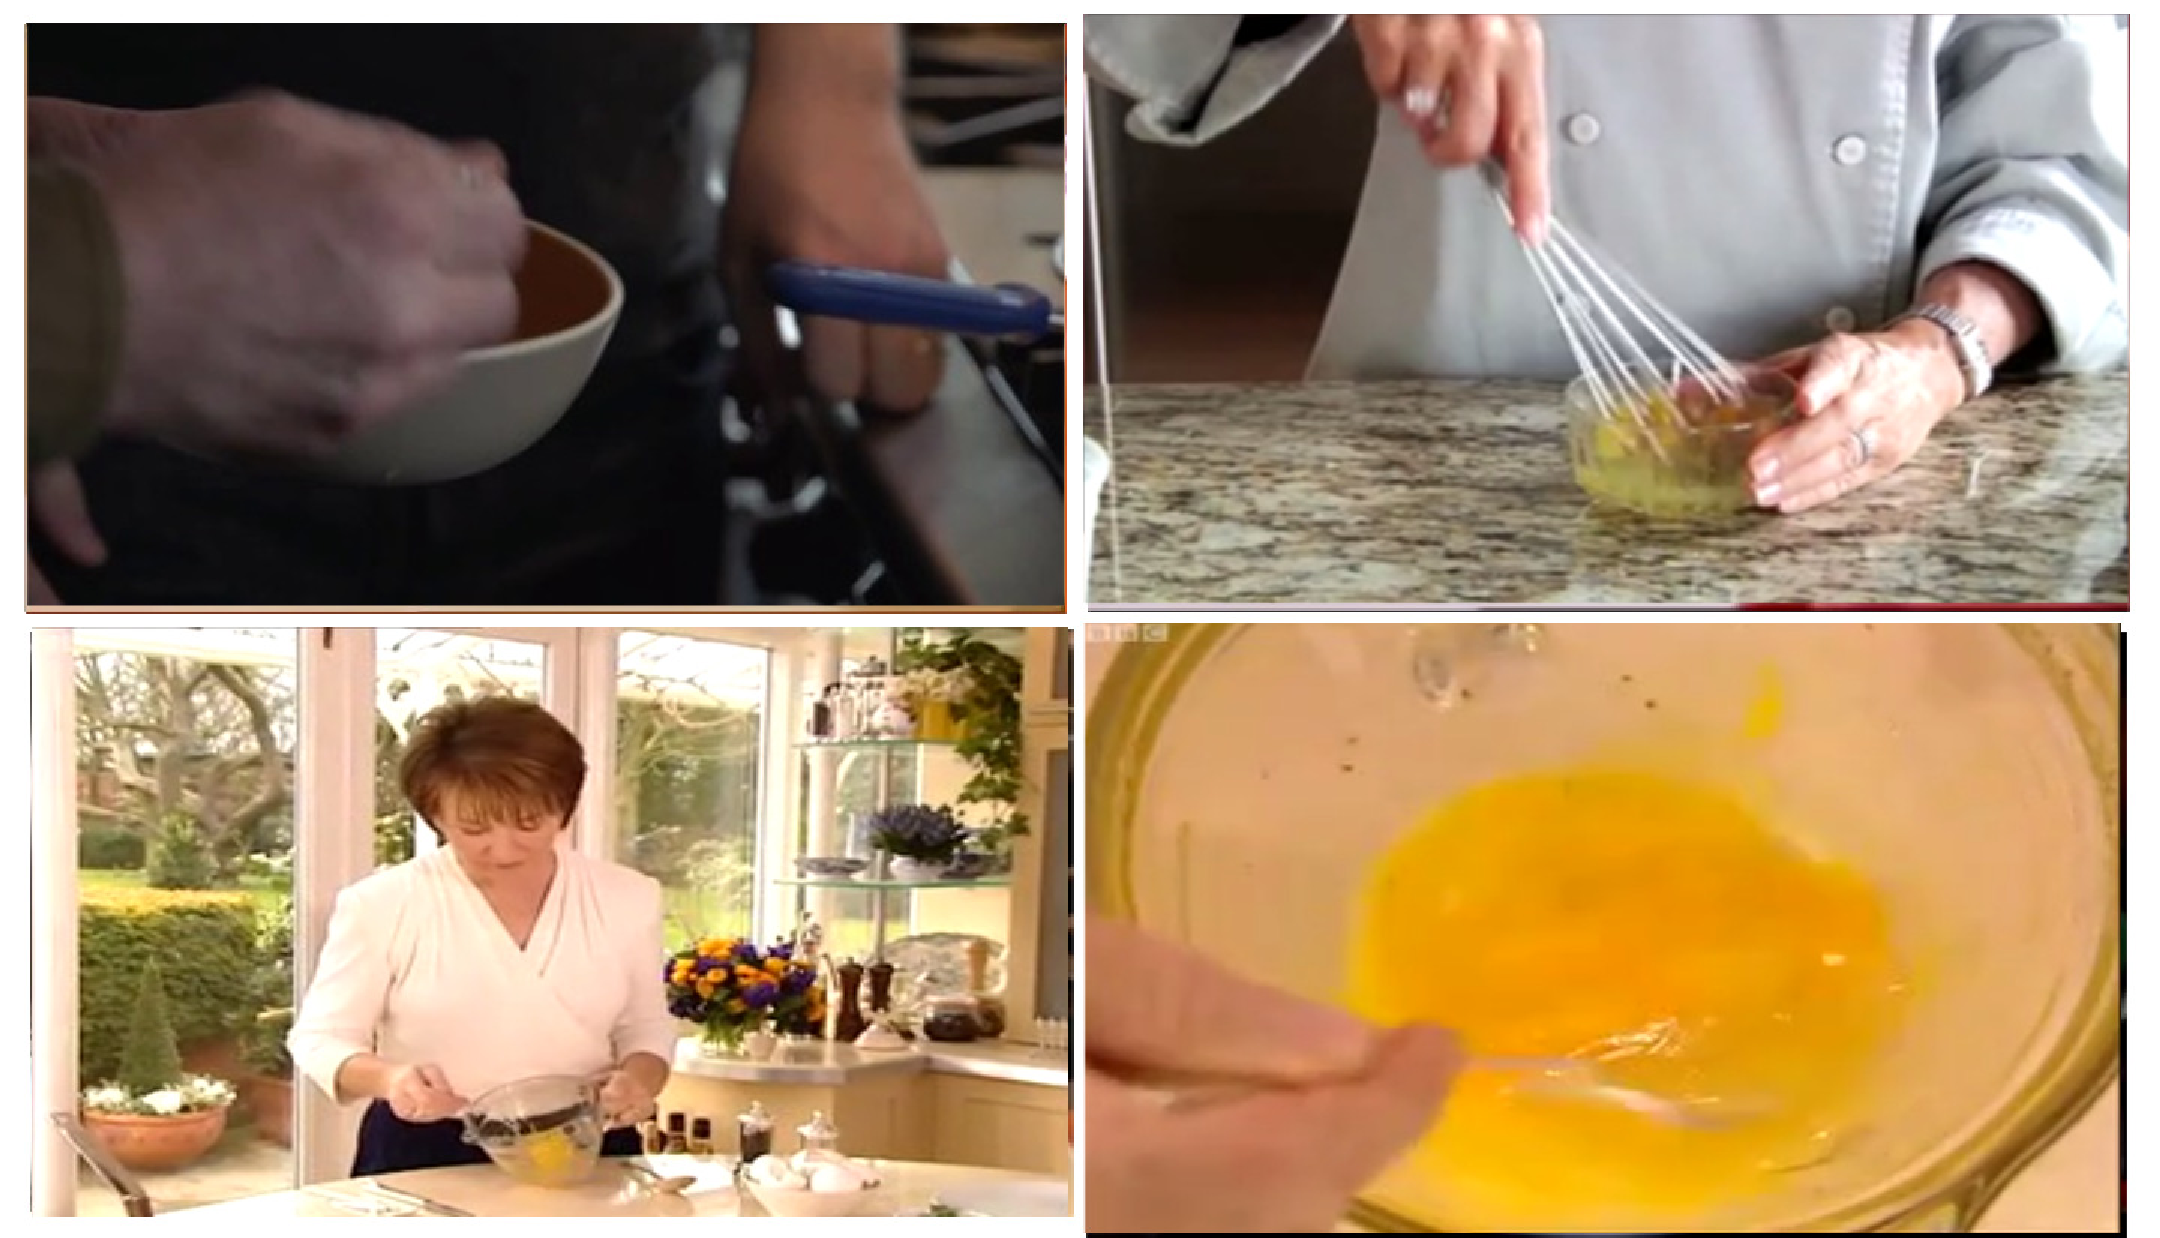
\includegraphics[width=\textwidth]{corange}
\color[HTML]{FF9900}{You can either use a fork or wire whisk to beat the eggs into a bowl.}
\end{subfigure}~
\begin{subfigure}[b]{0.5\textwidth}
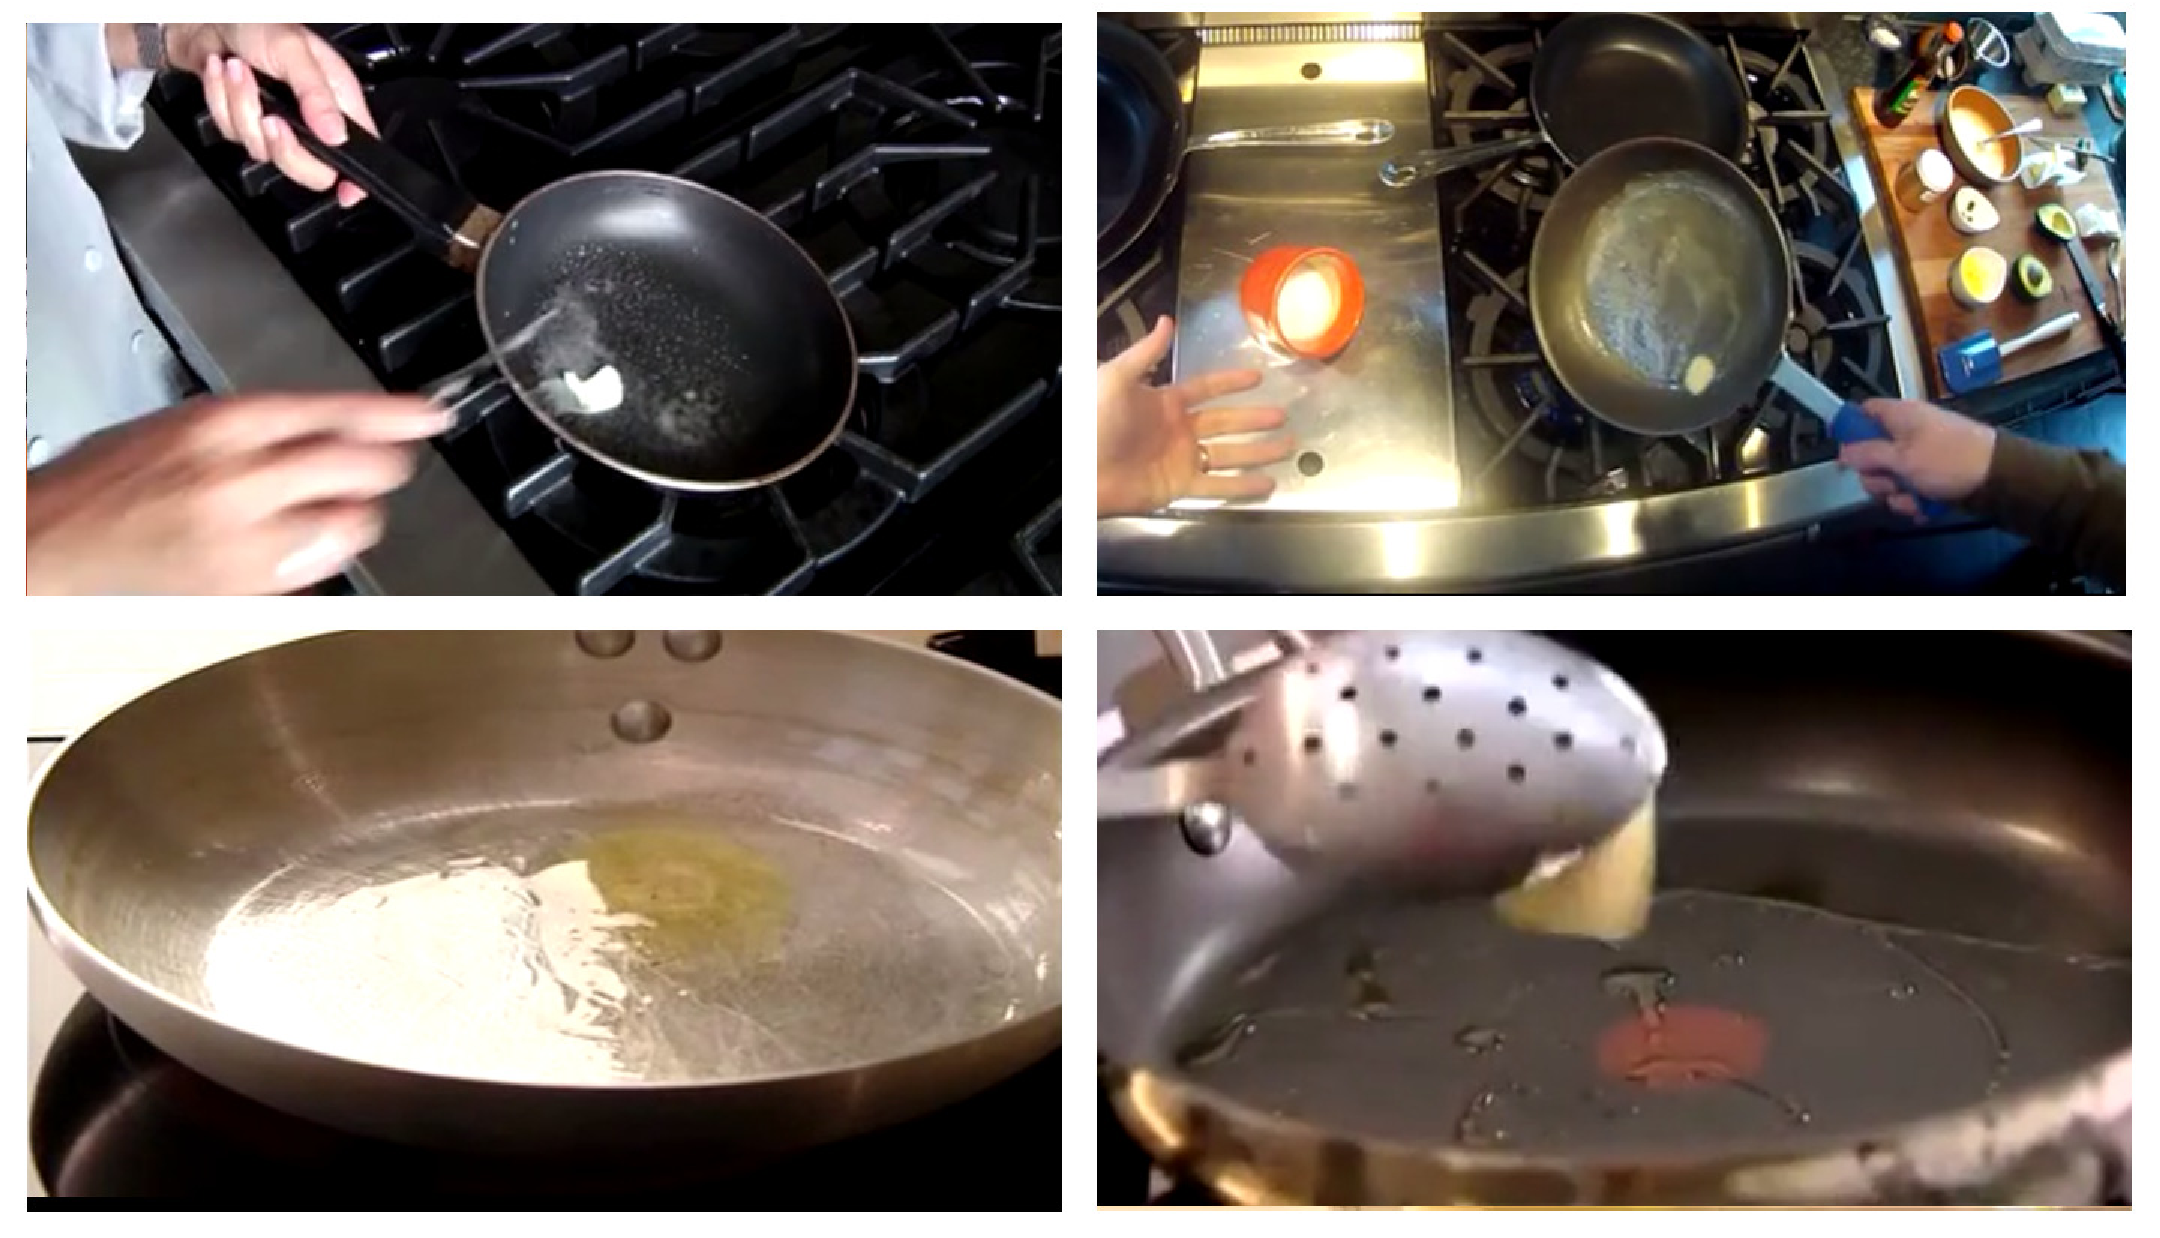
\includegraphics[width=\textwidth]{cgreen}
\color[HTML]{9DFF00}{Eggs cook quickly, so make sure the pan gets very hot first; the butter melt completely.}
\end{subfigure}



\caption{Sample images and the automatically generated captions for some of the clusters.}
\end{subfigure}

\end{figure}

\subsection{Quantitative Results}
\subsubsection{Baselines}
\paragraph{K-Means with low-level features:}
\paragraph{K-Means with semantic features:}
\paragraph{HMM with low-level features:}
\paragraph{HMM with semantic features:}
\paragraph{BP-HMM with low-level features:}
\paragraph{Category specific summary\cite{potapov2014category}:}


\subsubsection{Metrics}
\paragraph{Maximum Intersection over Union (M-IOU):}
\paragraph{Maximum Average Precision (M-AP):}
\paragraph{Semantic Correctness:}

\subsubsection{Results}
\paragraph{Are the activities detected accurately?}
\paragraph{Are the same activities in different videos linked to each other?}
\paragraph{Semantics vs Syntax:}
\paragraph{How important is each modality?}
\paragraph{Is joint clustering helpful?}
